\documentclass{article}

\usepackage[french]{babel}
\usepackage[utf8]{inputenc}
\usepackage[T1]{fontenc}
\usepackage{amsmath}
\usepackage{graphicx} %package to manage images
\usepackage[top=2cm,bottom=2cm]{geometry}
%%%%%%%%%%%%%%%% Lengths %%%%%%%%%%%%%%%%
\setlength{\textwidth}{15.5cm}
\setlength{\evensidemargin}{0.5cm}
\setlength{\oddsidemargin}{0.5cm}

%%%%%%%%%%%%%%%% Variables %%%%%%%%%%%%%%%%
\def\projet{3}
\def\titre{Compression d’image par l’algorithme de décomposition SVD}
\def\groupe{4}
\def\equipe{12472}
\def\responsible{Hector Piteau}
\def\secretary{Enzo Medina}
\def\others{Charles Wang, Dylan Machado}

\begin{document}

%%%%%%%%%%%%%%%% Header %%%%%%%%%%%%%%%%
\noindent\begin{minipage}{0.98\textwidth}
  \vskip 0mm
  \noindent
  { \begin{tabular}{p{7.5cm}}
      {\bfseries \sffamily
        Projet \projet} \\ 
      {\itshape \titre}
    \end{tabular}}
  \hfill 
  \fbox{\begin{tabular}{l}
      {~\hfill \bfseries \sffamily Groupe \groupe\ - Equipe \equipe
        \hfill~} \\[2mm] 
      Responsable : \responsible \\
      Secrétaire : \secretary \\
      Codeurs : \others
    \end{tabular}}
  \vskip 4mm ~

  ~~~\parbox{0.95\textwidth}{\small \textit{Résumé~: Dans ce projet, on cherche à compresser une image par utilisation de méthodes matricielles basée sur la factorisation SVD. Il est segmenté en quatre parties. \\
  Les trois premières permettent de transformer une matrice A (notre matrice contenant des triplets RGB) en un produit de 3 matrices : ${A = U*S*D}$. \\
  La dernière partie montre l'exploitation des algorithmes précédents sur une image.
    } \sffamily  }
  \vskip 1mm ~
\end{minipage}


%%%%%%%%%%%%%%%% Main part %%%%%%%%%%%%%%%%
\section{Transformations de Householder}

La première étape pour réaliser la compression d'une image est la construction d'une matrice de Householder $H$ qui permet de transformer un vecteur $X$ en un vecteur $Y$, i.e, $HX=Y$. Les vecteurs $X$ et $Y$ sont de même taille et de même norme.
Pour calculer $H$, on calcule: 
\begin{equation}
\begin{split}
        U = \frac{X-Y}{||X-Y||}\\
        H = Id - 2*U*U^T 
\end{split}
\end{equation}
Par exemple, pour $X$ = $\begin{pmatrix} 3 & 4 & 0\end{pmatrix}$
et $Y$ = $\begin{pmatrix}0 & 0 & 5\end{pmatrix}$,
$H$ vaut 
$\begin{pmatrix}
0.64 & -0.48 & 0.6\\
-0.48 & 0.36 & 0.8\\
0.6 & 0.8 & 0
\end{pmatrix}$.

On réutilisera ensuite cette matrice dans les deux prochaines parties. \\

Dans un premier temps, on développe un algorithme "naïf". On implémente donc simplement le calcul défini précédemment en prenant les vecteurs $X$ et $Y$ comme paramètres de l'algorithme.  
Soit $n$ la taille du vecteur, on a alors une complexité égale à ${O(n^2)}$ au vu des calculs de produit de matrices. \\

Pour optimiser l'algorithme précédent, on raisonne cette fois-ci en calculant en même temps le produit matriciel: 
\begin{equation}
\begin{split}
\alpha=U.V\\
HV = V - 2*\alpha*U 
\end{split}
\end{equation}
le produit scalaire entre le vecteur $U$ et $V$.
Il n'y a alors plus besoin de calculer un produit matriciel supplémentaire mais cela nécessite un nouveau vecteur $V$ en tant que nouveau paramètre de l'algorithme. 
La complexité est alors de ${O(4n)}$, soit une complexité équivalente à du ${O(n)}$. \\

Étant donné que l'on souhaite effectuer ces transformations de Householder sur plusieurs vecteurs, il est maintenant nécessaire de généraliser l'algorithme. 
Le vecteur $V$ est remplacé par une matrice $M$ de taille $(n, m)$ contenant $n$ vecteurs de taille $m$ et on exécute l'algorithme optimisé sur chaque ligne de la matrice. 
La complexité est donc multiplié par $n$ soit une complexité ${O(n^2)}$. \\

Afin de vérifier que notre deuxième algorithme est bien optimisé par rapport au premier, nous avons mesuré la durée de calcul sur des vecteurs de taille $n=10000$ pour les deux algorithmes.
L'algorithme non optimisé prend environ 2s alors que le deuxième prend environ 0.2ms. L'algorithme optimisé est donc 1000 fois plus rapide que la version non optimisé.
   
\section{Mise sous forme bidiagonale} 
   
\section{Transformations QR}

Après avoir mis notre matrice de pixels sous forme bidiagonale (à savoir la relation $A = Q_{left} \cdot BD \cdot Q_{right}$ où BD est la matrice bidiagonale), on va à présent mettre la matrice BD sous forme SVD en utilisant la décomposition QR. Pour cela, on commence par implémenter l'algorithme fourni dans le sujet en utilisant la fonction de numpy soit \textit{numpy.linalg.qr}.
\begin{enumerate}
    \item Écrire une version préliminaire de cet algorithme en utilisant la fonction numpy.linalg.qr.
    \item Tester et dessiner la convergence de la matrice S vers une matrice diagonale, et s’assurer que l’invariant$ U\times S\times V = BD$ est toujours vérifié.\\
    \newline
Les appels à la fonction de décomposition QR dans cet algorithme sont en fait disproportionnés : les matrices sur lesquelles on applique cet algorithme sont beaucoup plus simples que des matrices pleines.
    \item Montrer l’invariant suivant du calcul : « les matrices S, $R_1$ et $R_2$ sont toujours bidiagonales ».
    \item Réécrire une version simplifiée de la transformation QR en utilisant l’algorithme vu en cours et l’invariant précédent, puis utiliser cette optimisation pour votre algorithme de décomposition SVD. Quelles sont les complexités des deux algorithmes obtenus ?
    \item Usuellement, la décomposition SVD demande à ce que les éléments de la matrice S soient positifs, ordonnés de manière décroissante. Modifier les matrices U et S de manière à assurer cette propriété.
\end{enumerate}






\section{Application à la compression d’image}

Nous souhaitons maintenant compresser une image avec à l'aide des algorithmes précédents.
On note $k$ le rang de compression de l'image.
Pour compresser une image, on effectue les étapes suivantes : \\
\begin{enumerate}
    \item On convertit l'image en une matrice. Sur Python, la matrice résultante est une matrice de même taille que l'image dont les coefficients sont un triplet RGB représentant les couleurs rouge, bleu et vert. 
    \item On extrait de la matrice image les trois matrices de couleurs et on leur applique la décomposition SVD. 
    \item On annule les coefficient de la diagonale de $S$ au delà du $k$-ième coefficient et on compose les matrices de couleurs approchées.
    \item On recompose l'image à l'aide de ces matrices de couleurs.\\
\end{enumerate}

La matrice diagonale $S$ a ses coefficients diagonaux nuls après le $k$-ième coefficient.
On a réduit la taille de stockage de la matrice.
En effet, en notant $(n,m)$ la taille de la matrice image, au lieu de stocker $nm$ éléments, on en stocke que $2kn+k$ éléments ce qui est un gain considérable de place. \\
    

\begin{figure}[h]
   	\centering
%   	\begin{minipage}[c]{\linewidth}
   		\begin{minipage}[b]{0.25\linewidth}
		\centering 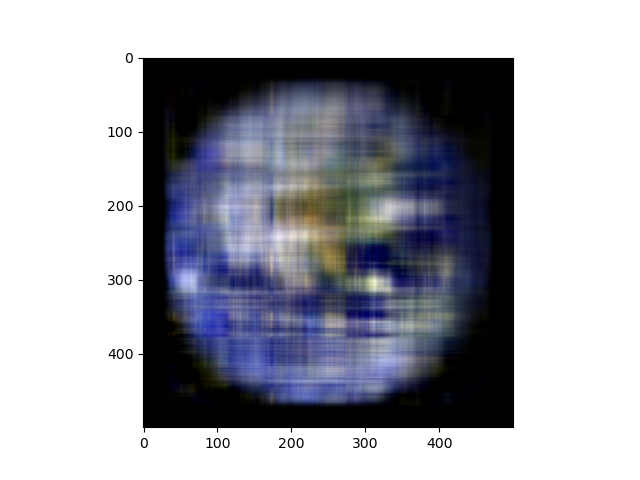
\includegraphics[height=3cm]{compress_5}
		\caption{$k=5$}
	\end{minipage}
		\begin{minipage}[b]{0.25\linewidth}
		\centering 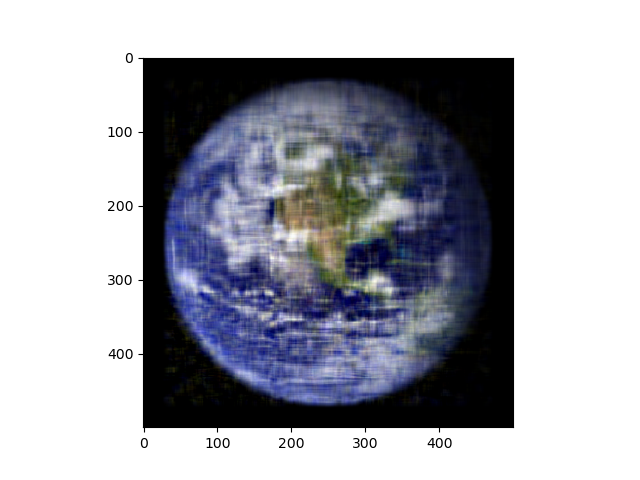
\includegraphics[height=3cm]{compress_15}
		\caption{$k=15$}
	\end{minipage}
		\begin{minipage}[b]{0.25\linewidth}
		\centering 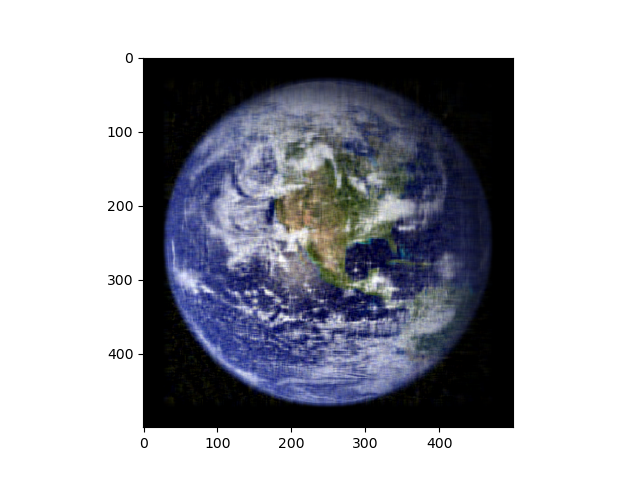
\includegraphics[height=3cm]{compress_30}
		\caption{$k=30$}
	\end{minipage}\hfill
%   		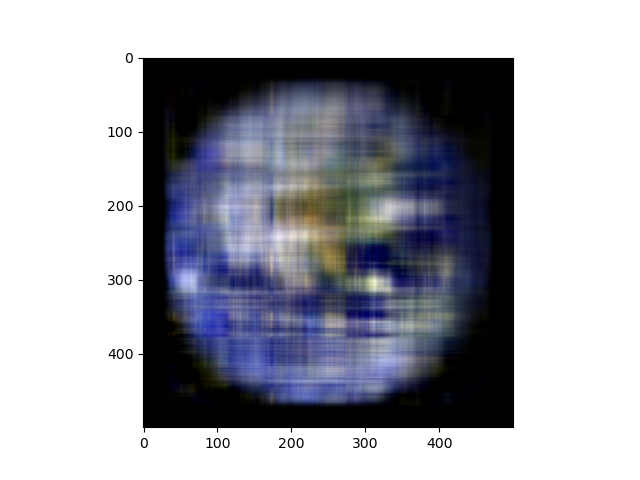
\includegraphics[height=3cm]{compress_5}
%   		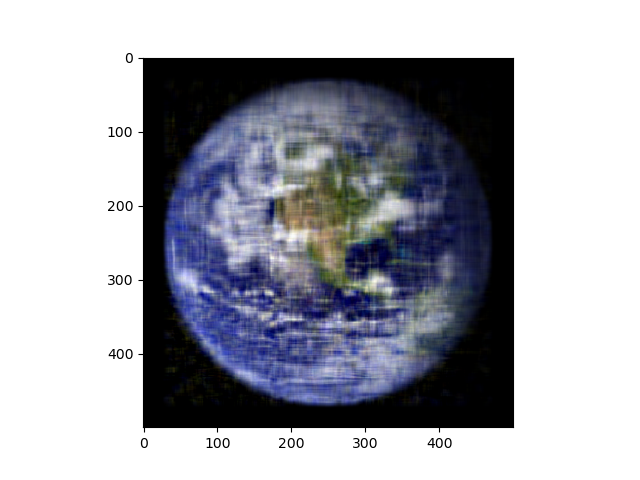
\includegraphics[height=3cm]{compress_15}
%   		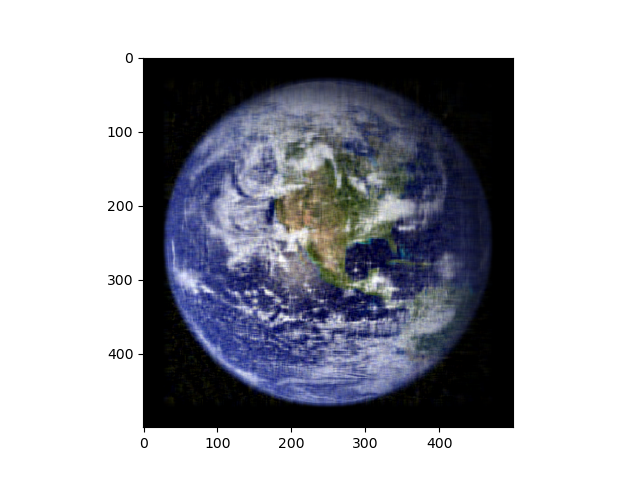
\includegraphics[height=3cm]{compress_30}
   	\caption{Illustrations de la compression SVD avec pour différents valeurs de $k$ }
   	\label{centre}
%     \end{minipage} \hfill 
\end{figure}

Pour mesurer ce gain, on se propose de calculer la distance euclidienne entre l'image normale et l'image compressée en fonction du rang $k$ de compression. Voici la comparaison obtenue en utilisant la factorisation SVD de la librairie numpy sur l'image de la fusée : \\

\begin{figure}[h]
    \centering 
    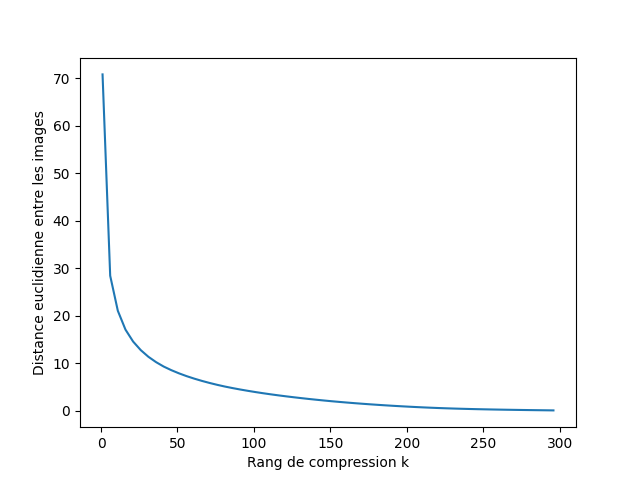
\includegraphics{distance}
    \caption{Distance euclidienne entre l'image normale et l'image compressée en fonction du rang de compression}
    \label{distance}
\end{figure}

On peut voir d'après notre graphique  que l'image compressée est très différente dès lors que k est faible (compris entre 0 et 25). La différence s'amenuise rapidement ce qui conduit à des images quasiment identiques à partir de k supérieur à 50.

%%%%%%%%%%%%%%%% End part %%%%%%%%%%%%%%%%
\section{Conclusion et apports du projet}
\paragraph{}

Ce projet nous a permis de découvrir une première approche des images en langage de programmation. Il nous a également permis de nous familiariser avec la factorisation SVD et les méthodes matricielles associés ainsi que les méthodes de compression d'image. Enfin, manipuler des images et donc pouvoir un visuel sur notre travail a été un véritable plaisir pour toute l'équipe. 


\end{document}

